% Typestate Programming

\begin{frame}[fragile,t]{Typestate Programming I}
    Den State mit dem Typ darstellen.
    \note<1>{
        \begin{itemize}
            \item Ein Konzept mit der State über den Typ einer variable dargestellt wird.
            \item So können die verschiedenen States und deren Übergänge viel besser Kontrolliert(eingeschränkt) werden.
            \item Es können sich auch die verfügbaren Methoden je nach State ändern.
        \end{itemize}
    }

    \pause Beispiel:
    \begin{figure}
        \centering
        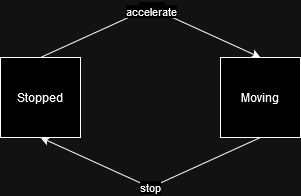
\includegraphics{images/typestate.drawio}
        \caption{Typestate Visualisierung}
        \label{fig:typestate-programming-1}
    \end{figure}

    \note<2>{
        \begin{itemize}
            \item Hier sehen wir das Konzept Visualisiert
            \item Wir haben zwei States: Stopped Moving
            \item Stopped ist der initial-State der mit new() erstellt werden kann
            \item Danach kann mit accelerate und stop\_after kontrolliert zwischen den States gewechselt werden
        \end{itemize}
    }

\end{frame}

\begin{frame}[fragile,t]{Typestate Programming II}
    State "Stopped" initialisieren:
    \begin{lstlisting}[language=Rust,escapechar=@,label={lst:typestate-programming-2-1}]
let car_state: Stopped = Stopped::new();
println!("Starting at {} m", car_state.get_distance());
\end{lstlisting}
    \codeoutput{code/04-typestate1.txt}

    \note<1>{
        \begin{itemize}
            \item Hier sehen wir wie mit der associatierten Funktion "new" eine instanz von Stopped erstellt wird
            \item Initial hat Stopped immer eine distance von 0, die Distanz kann nur durch den wechsel durch die States angepasst werden
        \end{itemize}
    }

    \pause zu State "Moving" übergehen
    \begin{lstlisting}[language=Rust,escapechar=@,label={lst:typestate-programming-2-2}]
let new_car_state: Moving = car_state.accelerate(
    5, // acceleration in m/s^2
    2 // how long to accelerate in seconds
);
println!("Accelerated to {} m/s", new_car_state.get_velocity());
\end{lstlisting}
    \codeoutput{code/04-typestate2.txt}

    \note<2> {
        \begin{itemize}
            \item Stopped hat die Funktion "accelerate", welche eine Instanz von "Moving" zurückgibt
            \item Dies ist der einzige Weg wie der State "Moving" erreicht werden kann
            \item Moving hat eine geschwindigkeit, die ausgelesen werden kann
        \end{itemize}
    }
\end{frame}



\begin{frame}[fragile,t]{Typestate Programming III}
    zurück zum State "Stopped"
    \begin{lstlisting}[language=Rust,escapechar=@,label={lst:typestate-programming-3-1}]
let final_car_state: Stopped = new_car_state.stop_after(
    10 // after how many seconds to stop moving
);

println!("Reached destination at {} m", final_car_state.get_distance());
    \end{lstlisting}
    \codeoutput{code/04-typestate3.txt}

    \note{
        \begin{itemize}
            \item Schlussendlich kann mit stop\_after wieder zum State Stopped zurückgekehrt werden
            \item Jetzt hat sich die Distanz erhöht, da für eine gewisse Zeit mit einer gewissen Geschwindigkeit bewegt wurde
            \item Die kann in Rust sehr einfach implementiert werden, da die Typisierung strict ist
            \item Dadurch dass es keine Vererbung gibt, kann auch nicht einfach ein CustomMoving State erstellt werden
        \end{itemize}
    }
\end{frame}
